\documentclass{beamer}
\usetheme{Boadilla}

\usepackage{standalone}
\usepackage[table]{xcolor}

\usepackage{fontspec}
\setmainfont{Times New Roman}

\usepackage[ukrainian]{babel}

\usepackage{polyglossia}
\setdefaultlanguage{ukrainian}
\setotherlanguages{english}
\setmonofont{Fira Code}[
  Scale=0.85
  ]
  \newfontfamily{\cyrillicfontsf}{Microsoft Sans Serif}

\usepackage{tikz}
\usepackage{pgfplots}
\usetikzlibrary{graphs,quotes}

\author{Кирило Байбула\\
        Науковий керівник:\\
        Самойленко Ігор Валерійович}
\date{\today}

\title{Знаходження оптимального шляху обміну у біржах на основі маркет мейкерів
  з функціями обміну константного добутку}

\institute{\textbf{КНУ ім. Тараса Шевченка}}

\date{\today}

\begin{document}

\begin{frame}
	\titlepage{}
\end{frame}

\begin{frame}\frametitle{Поняття резервів}
	\begin{columns}
		\begin{column}{.5\textwidth}
			\centering\textbf{$X$ = USD}

			\only<2>{
				\begin{tikzpicture}
					\node[rectangle,
						fill = blue!30!white,
						minimum width = 3cm,
						minimum height = 5cm,
						draw] (r) at (0,0) { $R_{X}$ = 100,000 \$};
				\end{tikzpicture}
			}
			\only<3>{
				\begin{tikzpicture}
					\node[rectangle,
						fill = blue!30!white,
						minimum width = 3cm,
						minimum height = 5cm,
						draw] (r) at (0,0) { $R_{X}$ = 100,100 \$};
					\node[rectangle,
						fill = green!30!white,
						minimum width = 3cm,
						minimum height = 0.5cm,
						draw] (r) at (0,2.75) { $+ \Delta x$ = 100 \$};
				\end{tikzpicture}
			}
		\end{column}
		\begin{column}{.5\textwidth}
			\centering\textbf{$Y$ = EUR}

			\only<2>{
				\begin{tikzpicture}
					\node[rectangle,
						fill = blue!30!white,
						minimum width = 3cm,
						minimum height = 5cm,
						draw] (r) at (0,0) { $R_{Y}$ = 110,000 €};
				\end{tikzpicture}
			}
			\only<3>{
				\begin{tikzpicture}
					\node[rectangle,
						fill = blue!30!white,
						minimum width = 3cm,
						minimum height = 5cm,
						draw] (r) at
					(0,0) { $R_{Y}$ = 109,890 €};
					\node[rectangle,
						fill = red!30!white,
						minimum width = 3cm,
						minimum height = 0.5cm,
						draw] (r) at (0,2.25) { $- \Delta y$ = 110 €};
				\end{tikzpicture}
			}
		\end{column}
	\end{columns}
	\vspace{2em}
\end{frame}

\begin{frame}\frametitle{Умови обміну}

	\begin{block}{Маркет мейкери константного добутку}
		Для $\Delta x$ - об'єм обміну валюти $X$, що користувач віддає, та $\Delta y$ - об'єм
		валюти $Y$, що користувач отримує, має виконується рівність:

		\begin{equation}\label{eq:exchange}
			R_{X} \cdot R_{Y} = (R_{X} + \Delta x) \cdot (R_{Y} - \Delta y)
		\end{equation}

		де $R_{X}, R_{Y}$ - резерви в парі $X/Y$.
	\end{block}

	У випадку коли умова \eqref{eq:exchange} виконується, обмін стається, інакше обмін не відбувається.
\end{frame}

\begin{frame}\frametitle{Граф біржі}
	\only<1>{
		\centering
		\begin{tikzpicture}
			\node[circle,draw = black] (x) at (0, -1) {X};
			\node[circle,draw = black] (y) at (4, 0) {Y};

			\draw[-] (x) to node [above, sloped] {} (y);
		\end{tikzpicture}
	}
	\only<2>{
		\centering
		\begin{tikzpicture}
			\node[circle,draw = black] (x) at (0, -1) {X};
			\node[circle,draw = black] (y) at (4, 0) {Y};
			\node[circle,draw = black] (z) at (8, 0) {Z};
			\node[circle,draw = black] (w) at (4, -2) {W};

			\draw[-] (x) to node [above, sloped] {} (y);
			\draw[-] (y) to node [above] {} (z);
			\draw[-] (x) to node [below,sloped] {} (w);
		\end{tikzpicture}
	}
	\only<3>{
		\begin{figure}
			\centering
			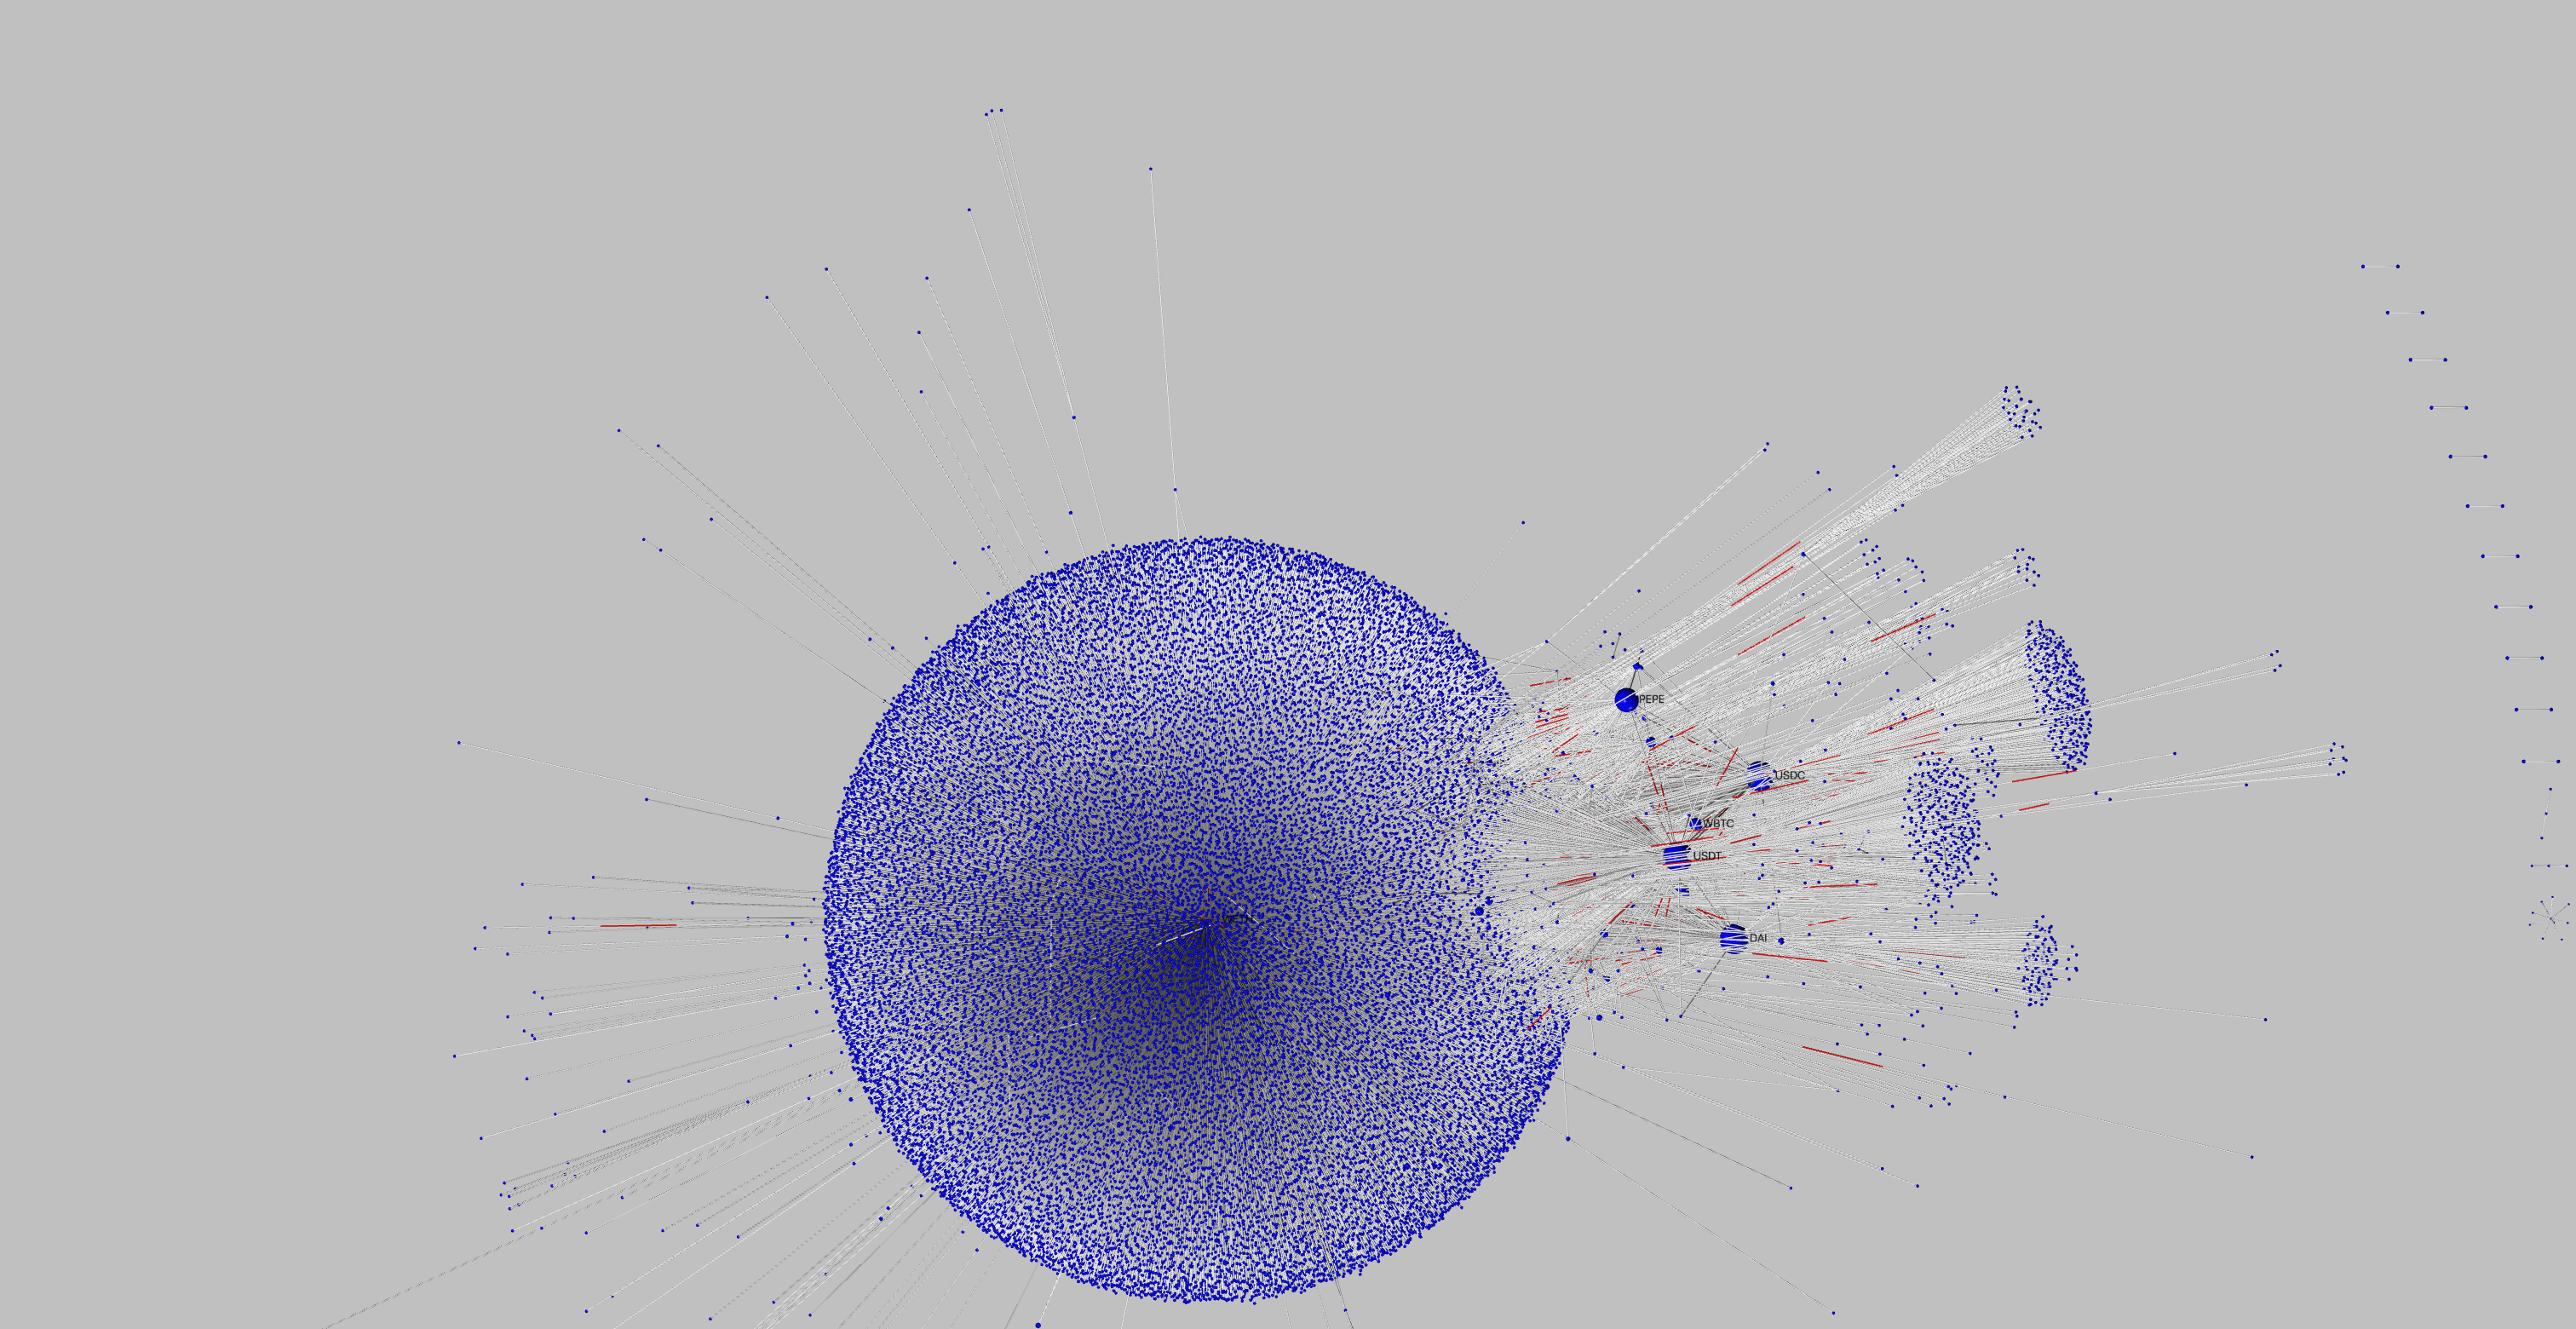
\includegraphics[scale=0.11]{presentation/images/graphia.png}
			\caption{Граф UniswapV2 з 250 тисяч ребер}
		\end{figure}
	}
\end{frame}

\begin{frame}\frametitle{Мета}
	\only<1>{
		\centering
		\begin{tikzpicture}
			% draw X at center
			\node[circle,draw = black] (x) at (0, 0) {X};

			% And place all other nodes around X
			\node[circle,draw = black] (y) at (2, 0) {Y};
			\node[circle,draw = black] (z) at (-2, 0) {Z};
			\node[circle,draw = black] (w) at (-2, 2) {W};
			\node[circle,draw = black] (v) at (2, 2) {V};
			\node[circle,draw = black] (u) at (0, 2) {U};
			\node[circle,draw = black] (t) at (0, -2) {T};
			\node[circle,draw = black] (s) at (4, 0) {S};
			\node[circle,draw = black] (r) at (-4, 0) {R};
			\node[circle,draw = black] (q) at (-4, 2) {Q};

			\node[circle,draw = black] (p) at (-2, -4) {P};
			\node[circle,draw = black] (o) at (2, -4) {O};

			% Draw edges for node around X
			\draw[-] (x) to node [above, sloped] {} (y);
			\draw[-] (x) to node [above, sloped] {} (z);
			\draw[-] (x) to node [above, sloped] {} (u);
			\draw[-] (x) to node [above, sloped] {} (t);;

			% Draw edges for node around Y
			\draw[-] (y) to node [above, sloped] {} (v);
			\draw[-] (y) to node [above, sloped] {} (s);

			% Draw edges for node around Z
			\draw[-] (z) to node [above, sloped] {} (w);
			\draw[-] (z) to node [above, sloped] {} (r);
			\draw[-] (z) to node [above, sloped] {} (q);

			% Draw edges for node around T
			\draw[-] (t) to node [above, sloped] {} (p);
			\draw[-] (t) to node [above, sloped] {} (o);

			% Draw other edges
			\draw[-] (w) to node [above, sloped] {} (u);
			\draw[-] (v) to node [above, sloped] {} (u);
			\draw[-] (u) to node [above, sloped] {} (s);
			\draw[-] (s) to node [above, sloped] {} (t);
			\draw[-] (r) to node [above, sloped] {} (t);
		\end{tikzpicture}
	}
	\only<2>{
		\centering
		\begin{tikzpicture}
			% draw X at center
			\node[circle,draw = red,text=red] (x) at (0, 0) {X};

			% And place all other nodes around X
			\node[circle,draw = black] (y) at (2, 0) {Y};
			\node[circle,draw = black] (z) at (-2, 0) {Z};
			\node[circle,draw = black] (w) at (-2, 2) {W};
			\node[circle,draw = black] (v) at (2, 2) {V};
			\node[circle,draw = black] (u) at (0, 2) {U};
			\node[circle,draw = black] (t) at (0, -2) {T};
			\node[circle,draw = black] (s) at (4, 0) {S};
			\node[circle,draw = black] (r) at (-4, 0) {R};
			\node[circle,draw = black] (q) at (-4, 2) {Q};

			\node[circle,draw = black] (p) at (-2, -4) {P};
			\node[circle,draw = black] (o) at (2, -4) {O};

			% Draw edges for node around X
			\draw[-] (x) to node [above, sloped] {?} (y);
			\draw[-] (x) to node [above, sloped] {?} (z);
			\draw[-] (x) to node [above, sloped] {?} (u);
			\draw[-] (x) to node [above, sloped] {?} (t);;
			% Draw edges for node around Y        ?
			\draw[-] (y) to node [above, sloped] {?} (v);
			\draw[-] (y) to node [above, sloped] {?} (s);
			% Draw edges for node around Z        ?
			\draw[-] (z) to node [above, sloped] {?} (w);
			\draw[-] (z) to node [above, sloped] {?} (r);
			\draw[-] (z) to node [above, sloped] {?} (q);
			% Draw edges for node around T        ?
			\draw[-] (t) to node [above, sloped] {?} (p);
			\draw[-] (t) to node [above, sloped] {?} (o);
			% Draw other edges                    ?
			\draw[-] (w) to node [above, sloped] {?} (u);
			\draw[-] (v) to node [above, sloped] {?} (u);
			\draw[-] (u) to node [above, sloped] {?} (s);
			\draw[-] (s) to node [above, sloped] {?} (t);
			\draw[-] (r) to node [above, sloped] {?} (t);
		\end{tikzpicture}
	}
\end{frame}

\begin{frame}\frametitle{Результати: Функція обміну}
	\begin{block}{Функція обміну}
		\begin{equation*}
			\Delta y = f_{X/Y}(\Delta x) = R_{Y} - \frac{R_{Y} R_{X}}{R_{X} + \gamma \Delta x}
		\end{equation*}
	\end{block}
	\pause{}
	\begin{block}{Композиція функцій обміну}
		\begin{equation*}
			f_{X/Y} \circ f_{Y/Z}  = f_{X/Y/Z}
		\end{equation*}
		\centering
		\begin{tikzpicture}
			\node (x) at (0, 0) {X};
			\node (y) at (2, 0) {Y};
			\node (z) at (4, 0) {Z};

			\draw[-] (x) to node [above] {$f_{X/Y}$} (y);
			\draw[-] (y) to node [above] {$f_{Y/Z}$} (z);
			\draw[bend right, -] (x) to node [below] {$f_{X/Y/Z}$} (z);
		\end{tikzpicture}
	\end{block}
\end{frame}

\begin{frame}\frametitle{Результати: Функція обміну для $n$ переходів}
	\begin{equation*}
		f_{C/\ldots/C_{i+1}} = f_{C_{0}/C_{1}} \circ f_{C_{1}/C_{2}} \circ \ldots f_{C_{i}/C_{i+1}}
	\end{equation*}
	\pause{}
	\begin{block}{Функція обміну для $n$ переходів}
		\begin{equation*}
			\begin{aligned}
				y & = (f_{C_{0}/C_{1}} \circ f_{C_{1}/C_{2}} \circ \ldots f_{C_{i}/C_{i+1}})(x) =                                                                                                \\
				  & = x \prod_{i=1}^n R_{C_{i+1}} \div \left( \prod_{i=1}^{n} R_{C_{i}} + x \sum_{i=0}^{n-1} \left( \prod_{k=1}^i R_{C_{i+1}} \cdot \prod_{j=i+2}^{n}  R_{C_{i}} \right) \right)
			\end{aligned}
		\end{equation*}
	\end{block}
\end{frame}

\begin{frame}\frametitle{Результати: Порівняння шляхів}
	\only<1>{
		\centering
		\begin{tikzpicture}
			% draw X at center
			\node[circle,draw = red,text=red] (x) at (0, 0) {X};

			% And place all other nodes around X
			\node[circle,draw = black] (y) at (3, 0) {Y};
			\node[circle,draw = black] (z) at (-2, 0) {Z};
			\node[circle,draw = black] (w) at (-2, 2) {W};
			\node[circle,draw = black] (v) at (2, 3) {V};
			\node[circle,draw = black] (u) at (0, 2) {U};
			\node[circle,draw = black] (t) at (0, -2) {T};
			\node[circle,draw = black] (s) at (5, 0) {S};
			\node[circle,draw = black] (r) at (-4, 0) {R};
			\node[circle,draw = black] (p) at (-2, -4) {P};
			\node[circle,draw = black] (o) at (2, -4) {O};

			\draw[-] (x) to node [above, sloped] {$f_{X/Y}$} (y);
			\draw[-] (x) to node [above, sloped] {$f_{X/Z}$} (z);
			\draw[-] (x) to node [above, sloped] {$f_{X/U}$} (u);
			\draw[-] (x) to node [above, sloped] {$f_{X/T}$} (t);
			\draw[-] (y) to node [above, sloped] {$f_{Y/V}$} (v);
			\draw[-] (y) to node [above, sloped] {$f_{Y/S}$} (s);
			\draw[-] (z) to node [above, sloped] {$f_{Z/W}$} (w);
			\draw[-] (z) to node [above, sloped] {$f_{Z/R}$} (r);
			\draw[-] (t) to node [above, sloped] {$f_{T/P}$} (p);
			\draw[-] (t) to node [above, sloped] {$f_{T/O}$} (o);
			\draw[-] (w) to node [above, sloped] {$f_{W/U}$} (u);
			\draw[-] (v) to node [above, sloped] {$f_{V/U}$} (u);
			\draw[-] (s) to node [above, sloped] {$f_{S/T}$} (t);
			\draw[-] (r) to node [above, sloped] {$f_{R/T}$} (t);
		\end{tikzpicture}
	}
	\only<2>{
		\centering
		\begin{tikzpicture}
			% draw X at center
			\node[circle,draw = red,text=red] (x) at (0, 0) {X};

			% And place all other nodes around X
			\node[circle,draw = black] (y) at (3, 0) {Y};
			\node[circle,draw = black] (v) at (5, 1) {V};
			\node[circle,draw = black] (s) at (5, -1) {S};

			% Draw edges for node around X
			\draw[->] (x) to node [above, sloped] {$f_{X/Y}$} (y);
			\draw[->] (y) to node [above, sloped] {$f_{Y/V}$} (v);
			\draw[->] (y) to node [above, sloped] {$f_{Y/S}$} (s);
		\end{tikzpicture}
	}
	\only<3>{
		\centering
		\begin{tikzpicture}
			% draw X at center
			\node[circle,draw = red,text=red] (x) at (0, 0) {X};

			% And place all other nodes around X
			\node[circle,draw = black] (y) at (3, 0) {Y};
			\node[circle,draw = black] (v) at (5, 1) {V};
			\node[circle,draw = black] (s) at (5, -1) {S};

			% Draw edges for node around X
			\draw[->] (x) to node [above, sloped] {$f_{X/Y}$} (y);
			\draw[->] (y) to node [above, sloped] {$f_{X/Y/V}$} (v);
			\draw[->] (y) to node [above, sloped] {$f_{X/Y/S}$} (s);
		\end{tikzpicture}
	}
	\only<4>{
		\centering
		\begin{tikzpicture}
			% draw X at center
			\node[circle,draw = red,text=red] (x) at (0, 0) {X};

			% And place all other nodes around X
			\node[circle,draw = black] (y) at (3, 0) {Y};
			\node[circle,draw = black] (v) at (5, 1) {V};
			\node[circle,draw = black] (s) at (5, -1) {S};

			\node[circle,draw = blue,text = blue] (base) at (2, 2) {\$};

			% Draw edges for node around X
			\draw[->] (x) to node [above, sloped] {$f_{X/Y/\$}$} (y);
			\draw[->] (y) to node [above, sloped] {$f_{X/Y/V/\$}$} (v);
			\draw[->] (y) to node [above, sloped] {$f_{X/Y/S/\$}$} (s);

			\draw[bend left=80, looseness=1.5, -, blue] (base) to node [above, sloped] {} (s);
			\draw[-, blue] (base) to node [above, sloped] {} (v);
			\draw[-, blue] (base) to node [above, sloped] {} (y);
			\draw[-, blue] (base) to node [above, sloped] {} (x);
		\end{tikzpicture}
	}
\end{frame}

\begin{frame}\frametitle{Результати: Алгоритм при фіксованому обʼємі $\Delta x$}
	\only<1>{
		Якщо $\Delta x$ - відоме значення обміну, то при обчисленні функцій
		отримуємо об'ємі після обмінів по шляхам графу в еквіваленті базової валюти
		(у даному випадку $\$$).

		\centering
		\begin{tikzpicture}
			% draw X at center
			\node[circle,draw = red,text=red] (x) at (0, 0) {X};

			% And place all other nodes around X
			\node[circle,draw = black] (y) at (3, 0) {Y};
			\node[circle,draw = black] (v) at (5, 1) {V};
			\node[circle,draw = black] (s) at (5, -1) {S};

			% Draw edges for node around X
			\draw[->] (x) to node [above, sloped] {$100 \$ $} (y);
			\draw[->] (y) to node [above, sloped] {$200 \$ $} (v);
			\draw[->] (y) to node [above, sloped] {$180 \$ $} (s);
		\end{tikzpicture}
	}
	\only<2>{
		\begin{equation*}
			f_{X/\$}(\Delta x) = 110 \$
		\end{equation*}
		\centering
		\begin{tikzpicture}
			% draw X at center
			\node[circle,draw = red,text=red] (x) at (0, 0) {X};

			% And place all other nodes around X
			\node[circle,draw = black] (y) at (3, 0) {Y};
			\node[circle,draw = black] (v) at (5, 1) {V};
			\node[circle,draw = black] (s) at (5, -1) {S};

			% Draw edges for node around X
			\draw[->] (x) to node [above, sloped] {$-10 \$ $} (y);
			\draw[->] (y) to node [above, sloped] {$+100 \$ $} (v);
			\draw[->] (y) to node [above, sloped] {$+80 \$ $} (s);
		\end{tikzpicture}
	}
	\only<3>{
		\centering
		\begin{tikzpicture}
			% draw X at center
			\node[circle,draw = red,text=red] (x) at (0, 0) {X};

			% And place all other nodes around X
			\node[circle,draw = black] (y) at (3, 0) {Y};
			\node[circle,draw = black] (z) at (-2, 0) {Z};
			\node[circle,draw = black] (w) at (-2, 2) {W};
			\node[circle,draw = black] (v) at (2, 3) {V};
			\node[circle,draw = black] (u) at (0, 2) {U};
			\node[circle,draw = black] (t) at (0, -2) {T};
			\node[circle,draw = black] (s) at (5.5, 0) {S};
			\node[circle,draw = black] (r) at (-4, 0) {R};
			\node[circle,draw = black] (p) at (-2, -4) {P};
			\node[circle,draw = black] (o) at (2, -4) {O};

			\draw[->] (x) to node [above, sloped] {$-10 \$$} (y);p
			\draw[->] (x) to node [above, sloped] {$+10 \$$} (z);
			\draw[->] (x) to node [above, sloped] {$+12 \$$} (u);
			\draw[->] (x) to node [above, sloped] {$-13 \$$} (t);
			\draw[->] (y) to node [above, sloped] {$+100 \$$} (v);
			\draw[->] (y) to node [above, sloped] {$+80 \$$} (s);
			\draw[->] (z) to node [above, sloped] {$+40 \$$} (w);
			\draw[->] (z) to node [above, sloped] {$-30 \$$} (r);
			\draw[->] (t) to node [above, sloped] {$+20 \$$} (p);
			\draw[->] (t) to node [above, sloped] {$-10 \$$} (o);
			\draw[->] (w) to node [above, sloped] {$+10 \$$} (u);
			\draw[->] (v) to node [above, sloped] {$+10 \$$} (u);
			\draw[->] (s) to node [above, sloped] {$+10 \$$} (t);
			\draw[->] (r) to node [above, sloped] {$+10 \$$} (t);

		\end{tikzpicture}
	}
\end{frame}

\begin{frame}
  \centering\Huge Дякую за увагу!
\end{frame}


\end{document}
